\chapter{Theoretical introduction}
	
\section{Problem introduction}
 Theoretical introduction to a problem and mathematical concepts, literature review.... \\
 
\noindent General task is to predict a weather state $\Omega_t$, observed at a timestamp $t$, given $s$ steps from the past, which are essentially previous weather states: $(\Omega_{t-1}, ..., \Omega_{t-s})$. We define $\Omega_t$ as a tensor of a shape: (latitude span, longitude span, features), therefore our complete input data would be 4-dimensional with additional dimension for a time \footnote{To be precise, for neural network based solutions it will be 5-dimensional due to the usage of batches.}. Spatial span was selected so as to cover the border of the whole of Poland and some of its neighbors. More details regarding data are discussed in dataset chapter~\ref{chap:dataset}. High-level spatio-temporal prediction framework is presented at Figure~\ref{fig:in_out}. \\

\noindent Forecasting performance would be evaluating by objective function:
\[
    \mathcal{L}(\hat{X}, X)
\]


\newpage
\subsection{Naming conventions and general prediction framework}
 For further convenience, we propose a general naming convention. 
 \begin{table}[!h]
    \centering
     \begin{tabular}{|c|c|}
        \hline
        Symbol & Description \\
        \hline
        $\mathbf{f}$ & Set of features: $(f_1,..., f_n)$ \\
        $s$ & Number of past steps \\
        $h$ & Forecasting horizon \\
        $\Omega$ & Weather state for all features \\
        $X_t$ & $\Omega$ for timestamp t\\
        $\mathbf{X}$ & $s$-element set of $\Omega$  \\
        $\hat{Y_t}$ & Prediction of $\Omega$ for timestamp t \\
        $\mathbf{\hat{Y}}$ & $h$-element set of predicted $\Omega$ \\
        $\hat{y_t}^{f_j}$ & Prediction of $\Omega$ for timestamp t and feature $f_j$ \\
        \hline
    \end{tabular}
    \caption{General conventions}
 \end{table}
 
 
%% \noindent We define a $\Phi$ as a set of baseline models that consist of: 
\begin{table}[!h]
    \centering
    \begin{tabular}{|c|c|}
        \hline
        Model Notation & Model Description \\
        \hline
        $\Phi_{es}$  & Exponential Smoothing \\
        $\Phi_{slr}$ & Simple Linear Regression \\
        $\Phi_{lr}$  & Linear Regression \\
        $\Phi_{gb}$ & Gradient Boosting Trees \\
        \hline
    \end{tabular}
\caption{Model conventions}
\end{table}
 
%% \noindent Additionally, due to the fact that model $\Phi_i$ consist of independent models that predicts single feature $f_j$ of a weather state, we can divide it into: 
 
 \noindent It is crucial to emphasize the fact that the scale of values of distinct features is diverse. Therefore, we define a model $\Phi_i$ as a collection of independent sub-models, each exclusively responsible for predicting distinct feature $f_j$. This solution was proposed to avoid situations in which the statistical dispersion of one feature might influence the prediction of another feature.  
 \[
 \Phi_{i} = (\Phi_{i}^{f_1}, ..., \Phi_{i}^{f_n})
 \]
 In further considerations, we will use a term: sub-models for each of $\Phi_{i}^{f_j}$.


\begin{figure}[!h]

\tikzset{every picture/.style={line width=0.75pt}} %set default line width to 0.75pt        

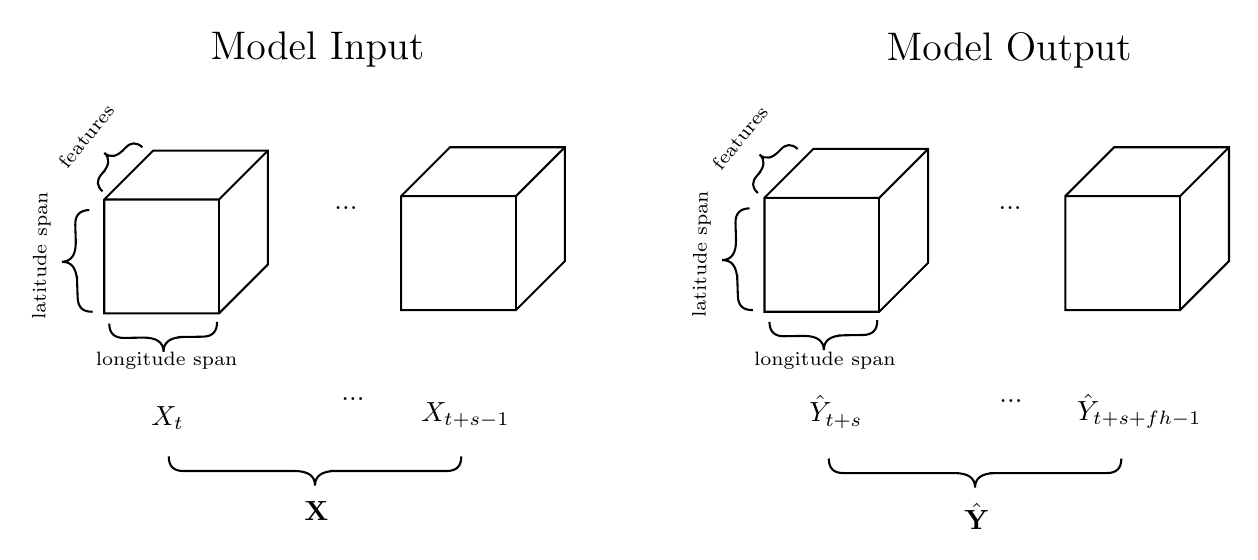
\begin{tikzpicture}[x=0.75pt,y=0.75pt,yscale=-1,xscale=1]
%uncomment if require: \path (0,389); %set diagram left start at 0, and has height of 389

%Shape: Cube [id:dp2816308175879604] 
\draw   (58.25,114.54) -- (81.78,91.01) -- (137.08,91.01) -- (137.08,145.91) -- (113.55,169.44) -- (58.25,169.44) -- cycle ; \draw   (137.08,91.01) -- (113.55,114.54) -- (58.25,114.54) ; \draw   (113.55,114.54) -- (113.55,169.44) ;
%Shape: Brace [id:dp4309828249836092] 
\draw   (76.63,89.37) .. controls (73.72,86.74) and (70.94,86.88) .. (68.31,89.8) -- (68.31,89.8) .. controls (64.55,93.97) and (61.21,94.73) .. (58.29,92.1) .. controls (61.21,94.73) and (60.79,98.13) .. (57.03,102.29)(58.72,100.42) -- (57.03,102.29) .. controls (54.4,105.21) and (54.54,107.99) .. (57.45,110.62) ;
%Shape: Brace [id:dp7756675475750493] 
\draw   (51.06,119.6) .. controls (46.39,119.75) and (44.14,122.16) .. (44.29,126.83) -- (44.53,134.35) .. controls (44.75,141.01) and (42.53,144.42) .. (37.86,144.57) .. controls (42.53,144.42) and (44.97,147.67) .. (45.19,154.34)(45.09,151.34) -- (45.43,161.86) .. controls (45.58,166.52) and (47.99,168.77) .. (52.66,168.62) ;
%Shape: Brace [id:dp612063156099937] 
\draw   (60.65,174.34) .. controls (60.72,179.01) and (63.09,181.3) .. (67.76,181.23) -- (76.73,181.09) .. controls (83.4,180.98) and (86.77,183.26) .. (86.84,187.93) .. controls (86.77,183.26) and (90.06,180.88) .. (96.73,180.78)(93.73,180.82) -- (105.71,180.64) .. controls (110.38,180.57) and (112.67,178.2) .. (112.6,173.53) ;
%Shape: Cube [id:dp42835259632452516] 
\draw   (201.31,112.9) -- (224.84,89.37) -- (280.14,89.37) -- (280.14,144.28) -- (256.61,167.81) -- (201.31,167.81) -- cycle ; \draw   (280.14,89.37) -- (256.61,112.9) -- (201.31,112.9) ; \draw   (256.61,112.9) -- (256.61,167.81) ;
%Shape: Brace [id:dp07592439753840141] 
\draw   (89.33,238.35) .. controls (89.33,243.02) and (91.66,245.35) .. (96.33,245.35) -- (149.81,245.35) .. controls (156.48,245.35) and (159.81,247.68) .. (159.81,252.35) .. controls (159.81,247.68) and (163.14,245.35) .. (169.81,245.35)(166.81,245.35) -- (223.29,245.35) .. controls (227.96,245.35) and (230.29,243.02) .. (230.29,238.35) ;
%Shape: Cube [id:dp7110500253196546] 
\draw   (376.35,113.72) -- (399.88,90.19) -- (455.18,90.19) -- (455.18,145.09) -- (431.65,168.62) -- (376.35,168.62) -- cycle ; \draw   (455.18,90.19) -- (431.65,113.72) -- (376.35,113.72) ; \draw   (431.65,113.72) -- (431.65,168.62) ;
%Shape: Brace [id:dp86120893233015] 
\draw   (392.33,90.19) .. controls (389.42,87.56) and (386.64,87.7) .. (384.01,90.62) -- (384.01,90.62) .. controls (380.25,94.78) and (376.91,95.54) .. (373.99,92.91) .. controls (376.91,95.54) and (376.49,98.94) .. (372.73,103.11)(374.42,101.24) -- (372.73,103.11) .. controls (370.1,106.02) and (370.24,108.8) .. (373.15,111.43) ;
%Shape: Brace [id:dp9673653209625941] 
\draw   (369.15,118.79) .. controls (364.49,118.94) and (362.24,121.34) .. (362.39,126.01) -- (362.63,133.53) .. controls (362.85,140.2) and (360.63,143.6) .. (355.96,143.75) .. controls (360.63,143.6) and (363.07,146.86) .. (363.28,153.52)(363.19,150.52) -- (363.53,161.04) .. controls (363.68,165.71) and (366.09,167.96) .. (370.75,167.81) ;
%Shape: Brace [id:dp9113296386668477] 
\draw   (378.74,173.53) .. controls (378.81,178.2) and (381.18,180.49) .. (385.85,180.42) -- (394.83,180.27) .. controls (401.5,180.17) and (404.87,182.45) .. (404.94,187.12) .. controls (404.87,182.45) and (408.16,180.07) .. (414.83,179.96)(411.83,180.01) -- (423.8,179.82) .. controls (428.47,179.75) and (430.76,177.38) .. (430.69,172.71) ;
%Shape: Cube [id:dp35039842919754816] 
\draw   (521.31,112.9) -- (544.84,89.37) -- (600.14,89.37) -- (600.14,144.28) -- (576.61,167.81) -- (521.31,167.81) -- cycle ; \draw   (600.14,89.37) -- (576.61,112.9) -- (521.31,112.9) ; \draw   (576.61,112.9) -- (576.61,167.81) ;
%Shape: Brace [id:dp3763157845274283] 
\draw   (407.33,239.35) .. controls (407.33,244.02) and (409.66,246.35) .. (414.33,246.35) -- (467.81,246.35) .. controls (474.48,246.35) and (477.81,248.68) .. (477.81,253.35) .. controls (477.81,248.68) and (481.14,246.35) .. (487.81,246.35)(484.81,246.35) -- (541.29,246.35) .. controls (545.96,246.35) and (548.29,244.02) .. (548.29,239.35) ;

% Text Node
\draw (33.24,96.31) node [anchor=north west][inner sep=0.75pt]  [rotate=-309.39,xslant=-0.03] [align=left] {{\scriptsize features}};
% Text Node
\draw (79.43,212.59) node [anchor=north west][inner sep=0.75pt]    {$X_{t}$};
% Text Node
\draw (167.65,116.51) node [anchor=north west][inner sep=0.75pt]   [align=left] {...};
% Text Node
\draw (21.86,173.65) node [anchor=north west][inner sep=0.75pt]  [rotate=-270.99] [align=left] {{\scriptsize latitude span}};
% Text Node
\draw (52.73,186.5) node [anchor=north west][inner sep=0.75pt]   [align=left] {{\scriptsize longitude span}};
% Text Node
\draw (209.49,210.96) node [anchor=north west][inner sep=0.75pt]    {$X_{t+s-1}$};
% Text Node
\draw (171.04,208.29) node [anchor=north west][inner sep=0.75pt]   [align=left] {...};
% Text Node
\draw (153.16,258.53) node [anchor=north west][inner sep=0.75pt]    {$\mathbf{X}$};
% Text Node
\draw (433.72,32.89) node [anchor=north west][inner sep=0.75pt]   [align=left] {{\Large Model Output}};
% Text Node
\draw (108.05,32.26) node [anchor=north west][inner sep=0.75pt]   [align=left] {{\Large Model Input}};
% Text Node
\draw (348.14,97.12) node [anchor=north west][inner sep=0.75pt]  [rotate=-309.39,xslant=-0.03] [align=left] {{\scriptsize features}};
% Text Node
\draw (339.95,172.84) node [anchor=north west][inner sep=0.75pt]  [rotate=-270.99] [align=left] {{\scriptsize latitude span}};
% Text Node
\draw (369.83,186.68) node [anchor=north west][inner sep=0.75pt]   [align=left] {{\scriptsize longitude span}};
% Text Node
\draw (487.65,116.51) node [anchor=north west][inner sep=0.75pt]   [align=left] {...};
% Text Node
\draw (396.43,207.59) node [anchor=north west][inner sep=0.75pt]    {$\hat{Y}_{t+s}$};
% Text Node
\draw (525.49,206.96) node [anchor=north west][inner sep=0.75pt]    {$\hat{Y}_{t+s+fh-1}$};
% Text Node
\draw (488.04,209.29) node [anchor=north west][inner sep=0.75pt]   [align=left] {...};
% Text Node
\draw (471.16,259.53) node [anchor=north west][inner sep=0.75pt]    {$\hat{\mathbf{Y}}$};


\end{tikzpicture}


\label{fig:in_out} \caption{Spatio-Temporal prediction framework} 

\end{figure}


\noindent Take into account the fact that this framework may differ when applying techniques such as grid neighbors~\ref{chap:neighbors} or using constants encodings~\ref{chap:feat_eng}. Details regarding those differences are explained deeply in subsequent chapters.

 \newpage
 
 \subsection{Literature review}
 After stating the problem we want to shortly inspect current research and results in this field... \\
Short review of quality papers related to this problem; explanation of what was already achieved in this task - SOTA solutions, especially emphasizing GraphCast paper; what we want to reproduce or compare ourself with. \\
\noindent Maybe start with: ~\cite{WFConsiderations}
MetNet, FourCastNet, GraphCast, and PanGu are state-of-the-art methods in the field of weather prediction.

\section{Explored techniques}
 \subsection{Autoregression}
 \noindent Each baseline model is designed to forecast the entire weather state for subsequent timestamp, with the forecasting horizon set at one. Therefore, when employing our models for short-term prediction tasks exceeding a few timestamps into the future, the autoregressive approach is commonsensical. \\ \\
 
 \noindent We denote model input as $\mathbf{X}$, a tensor of $s$ weather states: 
 \[
 \mathbf{X} = (X_{t}, ..., X_{t+s-1})
 \]
 and output of a model as $\mathbf{\hat{Y}}$, which consist of $h$ forecasted states:
 \[
 \mathbf{\hat{Y}} = (\hat{Y}_{t+s}, ..., \hat{Y}_{t+s+h-1})
 \]
 
 \noindent Autoregressive prediction is $h$-steps process such that:
 \begin{flalign*}
    &\hat{Y}_{t+s} = \Phi_{i}(X_{t}, ..., X_{t+s-1}) \\
    &\hat{Y}_{t+s+1} = \Phi_{i}(X_{t+1}, ..., X_{t+s-1}, \hat{Y}_{t+s}) \\
    &\vdots \\
    &\hat{Y}_{t+s+h-1} = \Phi_{i}(X_{t+h-1}, ...,  \hat{Y}_{t+s+h-3}, \hat{Y}_{t+s+h-2})
 \end{flalign*}

 \noindent Therefore, by simplifying:
 \[
    \mathbf{\hat{Y}} = \Phi_{i}(\mathbf{X})
 \]
 
 \noindent For each model except $\Phi_{slr}$, during every autoregressive step concatenation of outputs from sub-models is required, whereas $X_t$ needs to have information from every feature:
 \begin{flalign*}
    &\hat{y}_t^{f_j} = \Phi_{i}^{f_j}(\mathbf{X}_{t-1}) \\
    &\hat{Y}_{t} = (\hat{y}_t^{f_1}, ..., \hat{y}_t^{f_n}) \\
 \end{flalign*}
 
\subsection{Neighbors Extension}\label{chap:neighbors}

\noindent For every input tensor we have implemented an extension called additional neighbors. It expand each data points to include information about closely located grid boxes. Selection of neighbours is determined by the relative distance (radius) between the center of grid-boxes: $r$. In the illustration below, grey-colored grid boxes represents the primary data point and black boxes represents its neighbors. \\

\begin{figure}[!ht]
    \centering
    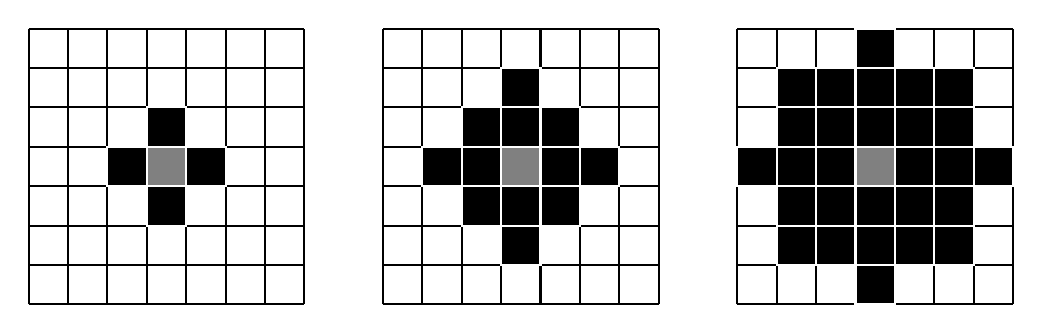
\begin{tikzpicture}[scale=0.5]
        \draw[step=1, black] (0,0) grid (7,7);
        \filldraw[fill=gray, draw=white] (3,3) rectangle (4,4);
        \filldraw[fill=black, draw=white] (3,2) rectangle (4,3);
        \filldraw[fill=black, draw=white] (2,3) rectangle (3,4);
        \filldraw[fill=black, draw=white] (3,4) rectangle (4,5);
        \filldraw[fill=black, draw=white] (4,3) rectangle (5,4);
        
        \begin{scope}[shift={(9,0)}]
            \draw[step=1, black] (0,0) grid (7,7);
            \foreach \i in {1, ..., 9} {
                \pgfmathtruncatemacro\row{mod(\i-1,3)}
                \pgfmathtruncatemacro\col{int((\i-1)/3)}
                \filldraw[fill=black, draw=white] (\row+2,\col+2) rectangle (\row+3,\col+3);
            }
            \filldraw[fill=gray, draw=white] (3,3) rectangle (4,4);
            \filldraw[fill=black, draw=white] (1,3) rectangle (2,4);
            \filldraw[fill=black, draw=white] (5,3) rectangle (6,4);
            \filldraw[fill=black, draw=white] (3,1) rectangle (4,2);
            \filldraw[fill=black, draw=white] (3,5) rectangle (4,6);
        \end{scope}

        \begin{scope}[shift={(18,0)}]
            \draw[step=1, black] (0,0) grid (7,7);
            \foreach \i in {1, ..., 25} {
                \pgfmathtruncatemacro\row{mod(\i-1,5)}
                \pgfmathtruncatemacro\col{int((\i-1)/5)}
                \filldraw[fill=black, draw=white] (\row+1,\col+1) rectangle (\row+2,\col+2);
            }
            \filldraw[fill=gray, draw=white] (3,3) rectangle (4,4); 
            \filldraw[fill=black, draw=white] (0,3) rectangle (1,4);
            \filldraw[fill=black, draw=white] (6,3) rectangle (7,4);
            \filldraw[fill=black, draw=white] (3,0) rectangle (4,1);
            \filldraw[fill=black, draw=white] (3,6) rectangle (4,7);
        \end{scope}
    \end{tikzpicture}
    \caption{Neighbors logic for $r=(1,2,3)$}
    \label{fig:neighbors}
\end{figure}

%Formal definition of a neighbors set $N$ for all of grid boxes $v$, where $V$ is a set of all:
\noindent Formal definition, assuming that grid boxes has resolution (1x1):
\begin{table}[!h]
    \centering
    \begin{tabular}{|c|c|}
        \hline
        Symbol & Description \\
        \hline
        $v_{i,j}$ & Grid box at latitude $i$ and longitude $j$ \\
        $V$  & Set of all grid boxes \\
        $\|v_{m,n} - v_{i,j}\|^2$  & Euclidian distance between centres of $v_{m,n}$ and $v_{i,j}$ \\
        $N_v$ & Set of neighbors for grid box $v$ \\
        \hline
    \end{tabular}
\end{table}
\[
    \forall v_{i,j} \in V: \{\forall v_{m,n \neq i,j} : \|v_{m,n} - v_{i,j}\|^2 \le r\} \in N_{v_{i,j}}
\]

\noindent Unfortunately, the trade-off between memory footprint, computational complexity, and performance gain was not sufficient to incorporate and test bigger $r$ values.

 
 \section{Baselines}
 \subsection{Exponential Smoothing}
 \subsection{Simple Linear Regression}\label{chap:slinear}
 This method is essentially a basic linear regression. When predicting a particular feature $f_i$, each sub-model only considers that specific feature in the input. It is a straightforward approach that assumes no correlation between different features and like any linear regression, it follows the basic assumptions of: linearity, independence, homoscedasticity, normality, absence of multicollinearity, and absence of endogeneity. Given that our task clearly deviates from meeting most of the mentioned assumptions, this method yields results that can be considered fairly average.
\begin{flalign*}
    &\forall f_i \in \mathbf{f}: \hat{y_t}^{f_i} = \Phi_{slr}^{f_i}(X_t^{f_i})\\
    &\hat{Y}_{t} = (\hat{y}_t^{f_1}, ..., \hat{y}_t^{f_n}) \\
\end{flalign*}

 \subsection{Linear Regression}\label{chap:linear}
It follows the same assumptions as \ref{chap:slinear}, but with a tweak. When forecasting the $f_i$ feature, it considers the complete weather state by using all available features as input. This indicate an assumption that different weather features might influence each other. While this approach is still naive linear model, it leads to slightly improved results. \\

  \noindent For both \ref{chap:slinear} and \ref{chap:slinear}, we have examined the performance of basic linear regression, as well as regularized versions - ridge, lasso, and elastic net. The outcomes indicate that ridge regression notably outperforms other methods. Further details are provided in the \ref{chap:report}rd chapter.
\begin{flalign*}
    &\forall f_i \in \mathbf{f}: \hat{y_t}^{f_i} = \Phi_{slr}^{f_i}(X_t)\\
    &\hat{Y}_{t} = (\hat{y}_t^{f_1}, ..., \hat{y}_t^{f_n}) \\
\end{flalign*}
\begin{table}[!h]
    \centering
    \begin{tabular}{|c|c|}
        \hline
        Method & Loss Function \\
        \hline
        Linear & $\sum(y_i - \hat{y_i})^2$ \\
        Ridge & $\sum(y_i - \hat{y_i})^2 + \lambda \sum w_j^2$ \\
        Lasso & $\sum(y_i - \hat{y_i})^2+ \lambda \sum |w_j|$ \\
        Elastic Net & $\sum(y_i - \hat{y_i})^2 +\lambda_1 \sum w_j^2 + \lambda_2 \sum |w_j|$  \\
        \hline
    \end{tabular}
\end{table}
 
 \[
    \mathbf{X} \boldsymbol\beta = \mathbf{\hat{Y}}
 \]

 \[
    \begin{bmatrix}
    x_{11} & x_{12} & \cdots & x_{1n}\\
    x_{21} & x_{22} & \cdots & x_{2n}\\
    \vdots & \vdots & \ddots & \vdots\\
    x_{n1} & x_{n2} & \cdots & x_{nn}
    \end{bmatrix}
    \begin{bmatrix}
    \beta_1\\\beta_2\\ \vdots\\b_n
    \end{bmatrix}
    =\begin{bmatrix}
    \hat{y_1}\\\hat{y_2}\\ \vdots\\\hat{y_n}
    \end{bmatrix}
\]
 \subsection{Gradient Boosting}
Due to the state-of-the-art performance in various tabular data-related challenges and their widespread popularity, we resolve to implement and analyze solutions based on gradient boosting algorithms. We chose two widely used methods, XGBoost ~\cite{Chen_2016} and LightGBM ~\cite{ke2017lightgbm}, both delivering improved results than other baseline methods. The fundamental idea behind gradient boosting lies in the iterative construction of multiple decision trees. Using the gradient boosting algorithm, these trees are generated to improve outcomes and create a more refined representation in each successive iteration. While XGBoost and LightGBM share multiple similarities, the primary distinction lies in their tree construction processes: leaf-wise for XGBoost and level-wise for LightGBM.  \\

\noindent We also explored CatBoost ~\cite{prokhorenkova2019catboost} and classical AdaBoost algorithms. However, due to significantly longer computation times and results that did not surpass other gradient boosting methods, we decided to exclude them from the further experiments and results comparison phase.

\section{Neural network concept}
Optional? \\

\noindent Explain architecture of dense neural networks and other types such as convolutional, recurrent, graph (depending on which one eventually will be used).

\section{GraphCast}
Deep dive into GraphCast architecture.

\section{Neural Network Models}
\subsection{UNet}
This might be consider baseline too but since achieving very high scores and sharing similar characteristics with gnn it might be described here.

\subsection{GNN}
Proposed model architecture and comparision with GraphCast. \\

\noindent After briefly testing multiple Graph Convolutional Cells that support edge feature vectors, we have concluded that the most promising results and sufficient computation time are obtained by TransformerConv ~\cite{shi2021masked}.\\

\noindent Multi-layer perceptron as an embedder converting features dimension into more abstract latent space that stores better representation of weather state.

.... \\

\noindent Multi-layer perceptron as a decoder converting encoded features into its natural representation.


\begin{flalign*}
    X = MLP^{Embedder}(X) \\
    X = GNN_1(X) \\
    ...         \\
    X = GNN_N(X) \\
    \hat{Y} = MLP^{Decoder}(X) \\
 \end{flalign*}

 \begin{flalign*}
    d_{V_i,V_j} &= \sqrt{(V_{j_x} - V_{i_x})^2 + (V_{j_y} - V_{i_y})^2} \\
    e_{V_i,V_j} &= (V_{j_x} - V_{i_x}, V_{j_y} - V_{i_y}, d_{V_i,V_j})
\end{flalign*}

\begin{figure}[!ht]

\centering


\tikzset{every picture/.style={line width=0.75pt}} %set default line width to 0.75pt        

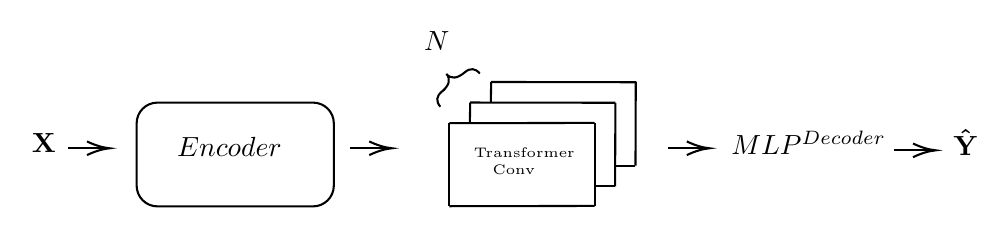
\begin{tikzpicture}[x=0.75pt,y=0.75pt,yscale=-1,xscale=1]
%uncomment if require: \path (0,300); %set diagram left start at 0, and has height of 300

%Shape: Brace [id:dp7019805664018027] 
\draw   (292.33,79) .. controls (290.14,76.39) and (287.74,76.19) .. (285.13,78.38) -- (285.13,78.38) .. controls (281.4,81.52) and (278.44,81.79) .. (276.25,79.18) .. controls (278.44,81.79) and (277.68,84.66) .. (273.95,87.79)(275.63,86.38) -- (273.95,87.79) .. controls (271.34,89.99) and (271.14,92.39) .. (273.33,95) ;
%Straight Lines [id:da24344825121139568] 
\draw    (277.63,102.92) -- (277.63,142.92) ;
%Straight Lines [id:da6110561454804792] 
\draw    (347.7,102.78) -- (347.7,142.78) ;
%Straight Lines [id:da03871795486024654] 
\draw    (277.63,102.92) -- (347.7,102.78) ;
%Straight Lines [id:da49608827752120055] 
\draw    (277.63,142.92) -- (347.7,142.78) ;
%Straight Lines [id:da27192408985546146] 
\draw    (287.69,92.96) -- (357.66,93.08) ;
%Straight Lines [id:da3480819733752343] 
\draw    (287.69,92.96) -- (287.55,102.87) ;
%Straight Lines [id:da3901687935554585] 
\draw    (297.79,83.06) -- (367.76,83.19) ;
%Straight Lines [id:da39197446094452226] 
\draw    (297.79,83.06) -- (297.66,92.98) ;
%Straight Lines [id:da01971233582821519] 
\draw    (357.52,133.35) -- (347.61,133.35) ;
%Straight Lines [id:da8552790800436195] 
\draw    (367.34,123.41) -- (357.43,123.41) ;
%Straight Lines [id:da901598531956911] 
\draw    (357.66,93.08) -- (357.52,133.35) ;
%Straight Lines [id:da7619590199519597] 
\draw    (367.48,83.15) -- (367.34,123.41) ;
%Straight Lines [id:da8643445648605664] 
\draw    (94,115) -- (112,115) ;
\draw [shift={(114,115)}, rotate = 180] [color={rgb, 255:red, 0; green, 0; blue, 0 }  ][line width=0.75]    (10.93,-3.29) .. controls (6.95,-1.4) and (3.31,-0.3) .. (0,0) .. controls (3.31,0.3) and (6.95,1.4) .. (10.93,3.29)   ;
%Straight Lines [id:da10221146771541123] 
\draw    (492,116) -- (510,116) ;
\draw [shift={(512,116)}, rotate = 180] [color={rgb, 255:red, 0; green, 0; blue, 0 }  ][line width=0.75]    (10.93,-3.29) .. controls (6.95,-1.4) and (3.31,-0.3) .. (0,0) .. controls (3.31,0.3) and (6.95,1.4) .. (10.93,3.29)   ;
%Straight Lines [id:da5913843902335524] 
\draw    (383,115) -- (401,115) ;
\draw [shift={(403,115)}, rotate = 180] [color={rgb, 255:red, 0; green, 0; blue, 0 }  ][line width=0.75]    (10.93,-3.29) .. controls (6.95,-1.4) and (3.31,-0.3) .. (0,0) .. controls (3.31,0.3) and (6.95,1.4) .. (10.93,3.29)   ;
%Rounded Rect [id:dp0019134800479860825] 
\draw   (127,103) .. controls (127,97.48) and (131.48,93) .. (137,93) -- (212,93) .. controls (217.52,93) and (222,97.48) .. (222,103) -- (222,133) .. controls (222,138.52) and (217.52,143) .. (212,143) -- (137,143) .. controls (131.48,143) and (127,138.52) .. (127,133) -- cycle ;
%Straight Lines [id:da4758105819320845] 
\draw    (230,115) -- (248,115) ;
\draw [shift={(250,115)}, rotate = 180] [color={rgb, 255:red, 0; green, 0; blue, 0 }  ][line width=0.75]    (10.93,-3.29) .. controls (6.95,-1.4) and (3.31,-0.3) .. (0,0) .. controls (3.31,0.3) and (6.95,1.4) .. (10.93,3.29)   ;

% Text Node
\draw (288,110) node [anchor=north west][inner sep=0.75pt]  [font=\tiny] [align=left] {\begin{minipage}[lt]{28.82pt}\setlength\topsep{0pt}
\begin{center}
{\tiny Transformer }\\{\tiny Conv}
\end{center}

\end{minipage}};
% Text Node
\draw (264,57.4) node [anchor=north west][inner sep=0.75pt]    {$N$};
% Text Node
\draw (412,105.4) node [anchor=north west][inner sep=0.75pt]    {$MLP^{Decoder}$};
% Text Node
\draw (75,106.4) node [anchor=north west][inner sep=0.75pt]    {$\mathbf{X}$};
% Text Node
\draw (519,104.4) node [anchor=north west][inner sep=0.75pt]    {$\mathbf{\hat{Y}}$};
% Text Node
\draw (145,108.4) node [anchor=north west][inner sep=0.75pt]    {$Encoder$};


\end{tikzpicture}


\caption{Architecture overview}
    \label{fig:architecture}
\end{figure}

\subsection{Additional techniques and feature engineering}\label{chap:feat_eng}
Present concept of spatial-mapping, edge attributes. Explain spatial and temporal feature encodings as well as usage of constants like geopotential. 

%% \subsubsection{Constant features}
\subsubsection{Spatio-Temporal embedder}
To build a better representation of the knowledge of the weather conditions, constant/exogenous features such as geopotential, and land-sea mask were also used as a model input. In addition, with the help of the so-called Spatio-Temporal embedder - $ST^{Embedder}$, we encoded spatial and temporal information, and concatenated it in the process of forward propagation with the input feature tensor, thus obtaining a better knowledge representation for individual grid-boxes. \\

\noindent The encodings for latitude and longitude (lat,lon) of each grid box / node $v_{i,j}$ are represented as:
\[
\mathbf{u}_{geo, v_{i,j}} =
\begin{bmatrix}
    \sin{2\pi\frac{lat}{180}} &
    \cos{2\pi\frac{lat}{180}} &
    \sin{2\pi\frac{lon}{360}} &
    \cos{2\pi\frac{lon}{360}}
\end{bmatrix}
\]

\noindent Encoding of time for entire model input at timestamp $t$, where $(d, h)$ represents the day of the year and the hour in a day, is given by:
\[
\mathbf{u}_{time,t} =
\begin{bmatrix}
    \sin{2\pi\frac{d}{365}} &
    \cos{2\pi\frac{d}{365}} &
    \sin{2\pi\frac{h}{24}} &
    \cos{2\pi\frac{h}{24}}
\end{bmatrix}
\]

\noindent In the subsequent analysis, we denote the product of latitude and longitude spans as $S$. It represents the flattened spatial dimension of tensors. $B$ stands for the batch size. \\ 

\noindent The concatenation of spatio-temporal features with weather features occurs right after the input tensor passes through the $MLP^{Embedder}$ and before entering graph cells. Following the dense layer, weather representation tensor has dimensions ($B$, $S$, hidden), the $\mathbf{u}_{time}$ tensor (batch, 1, 4), and the $\mathbf{u}_{geo}$ tensor ($B$, $S$, 4). To align the corresponding dimensions of $\mathbf{u}_{time}$ it goes through another dense layer with hidden size: $S$, from which it comes out having shape: ($B$, 1, $S$), after transposing the last two dimensions we will get ($B$, $S$, 1) and ability to concatenate all 3 tensors together creating one with shape: ($B$, $S$, hidden+4+1). The concatenated tensor passes through one more dense layer ultimetaly achieving the dimension ($B$, $S$, hidden') and creating a tensor aware of spatio-temporal context. Then, the forward propagatation through the graph cells of the network occurs.

\begin{center}
    \begin{tabular}{|l|l|}
        \hline
        \textbf{Operation} & \textbf{Output shape} \\
        \hline
        $X = MLP^{Embedder}(X)$ & $(B, S, \text{Hidden})$ \\
        $\mathbf{u}_{time} = Dense(\mathbf{u}_{time})^T$ & $(B, S, 1)$ \\
        $X = (X \oplus \mathbf{u}_{time} \oplus \mathbf{u}_{geo})$ & $(B, S, \text{Hidden} + 4 + 1)$ \\
        $X = Dense(X)$ & $(B, S, \text{Hidden'})$ \\
        \hline
    \end{tabular}
\end{center}

\subsubsection{Spatial-Mapping}
Spatial mapping was introduced to extinguish the influence of areas near the boundaries of the input space, which were detrimental to the quality of the prediction. In the original GraphCast architecture, the data spanned the enitre globe, creating a fully connected graph; where our model utilizes data from only a small part of the globe. As the result, vertices located on the space boundaries are connected only to the inner vertices, leading to lack of weather information. Hence, we decided that in the process of training, specifically in cost function computation, and model evaluation only a subspace of the model input is employed. The concept is illustrated in the figure, actual input dimensions are maintained.

\begin{figure}[!ht]
    \centering
    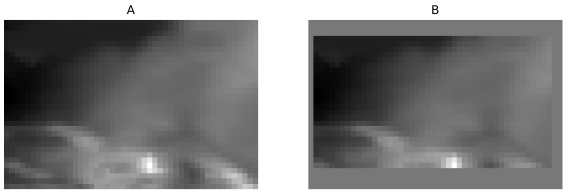
\includegraphics[scale=0.75]{figures/spatial_mapping.pdf}
    \caption{A: (32x48) Model input; B: (25x45) Mapped space}
    \label{fig:spatial_map}
\end{figure}
 

\noindent TODO: Better visualization